\documentclass[journal]{IEEEtran}

\usepackage{cite}
\usepackage{amsmath,amssymb,amsfonts}
\usepackage{algorithm}
\usepackage{algorithmic}
\usepackage{graphicx}
\usepackage{textcomp}
\usepackage{xcolor}
\usepackage{color}
\usepackage{bm}
\usepackage{subfigure}
\usepackage{booktabs}
%\documentclass[12pt, draftclsnofoot, onecolumn]{IEEEtran}
%
% If IEEEtran.cls has not been installed into the LaTeX system files,
% manually specify the path to it like:
% \documentclass[journal]{../sty/IEEEtran}


% *** GRAPHICS RELATED PACKAGES ***
%
\ifCLASSINFOpdf
  % \usepackage[pdftex]{graphicx}
  % declare the path(s) where your graphic files are
  % \graphicspath{{../pdf/}{../jpeg/}}
  % and their extensions so you won't have to specify these with
  % every instance of \includegraphics
  % \DeclareGraphicsExtensions{.pdf,.jpeg,.png}
\else
  % or other class option (dvipsone, dvipdf, if not using dvips). graphicx
  % will default to the driver specified in the system graphics.cfg if no
  % driver is specified.
  % \usepackage[dvips]{graphicx}
  % declare the path(s) where your graphic files are
  % \graphicspath{{../eps/}}
  % and their extensions so you won't have to specify these with
  % every instance of \includegraphics
  % \DeclareGraphicsExtensions{.eps}
\fi

\hyphenation{op-tical net-works semi-conduc-tor}


\begin{document}
%
% paper title
% Titles are generally capitalized except for words such as a, an, and, as,
% at, but, by, for, in, nor, of, on, or, the, to and up, which are usually
% not capitalized unless they are the first or last word of the title.
% Linebreaks \\ can be used within to get better formatting as desired.
% Do not put math or special symbols in the title.
\title{Learning-based Robust and Secure Transmission for Reconfigurable Intelligent Surface Aided Millimeter Wave UAV Communications}
%
%
% author names and IEEE memberships
% note positions of commas and nonbreaking spaces ( ~ ) LaTeX will not break
% a structure at a ~ so this keeps an author's name from being broken across
% two lines.
% use \thanks{} to gain access to the first footnote area
% a separate \thanks must be used for each paragraph as LaTeX2e's \thanks
% was not built to handle multiple paragraphs
%

\author{Xufeng~Guo,~Ying~Wang,~\IEEEmembership{Member,~IEEE,}~and~Yuanbin Chen% <-this % stops a space
	
\thanks{	
	\textit{Corresponding author: Ying Wang.}
	
	X. Guo, Y. Wang, and Y. Chen are with the State Key Laboratory of Networking and Switching Technology, Beijing University of Posts and Telecommunications, Beijing, China 100876 (e-mail:xxx; wangying@bupt.edu.cn; chen\_yuanbin@163.com).% <-this % stops a space
%\thanks{Manuscript received April 19, 2005; revised August 26, 2015.}
}}


% make the title area
\maketitle

% As a general rule, do not put math, special symbols or citations
% in the abstract or keywords.
\begin{abstract}
The abstract goes here.
\end{abstract}

% Note that keywords are not normally used for peerreview papers.
\begin{IEEEkeywords}
IEEE, IEEEtran, journal, \LaTeX, paper, template.
\end{IEEEkeywords}






% For peer review papers, you can put extra information on the cover
% page as needed:
% \ifCLASSOPTIONpeerreview
% \begin{center} \bfseries EDICS Category: 3-BBND \end{center}
% \fi
%
% For peerreview papers, this IEEEtran command inserts a page break and
% creates the second title. It will be ignored for other modes.
\IEEEpeerreviewmaketitle



\section{Introduction}
Millimeter-wave (mmWave) communications with multi-gigahertz bandwidth availability boost much higher capacity and transmission rate than conventional sub-6GHz communications. Unmanned aerial vehicles (UAVs), which are featured by their high mobility and flexible deployment, are promising candidates to compensate most of the deficiencies of mmWave signals, preserve its advantages, and provide more opportunities \cite{UAVMMWAVE-2}. However, the mmWave signals transmitted by UAVs are prone to deteriorate due to their high sensitivity to the presence of spatial blockages, especially in the complex propagation environment (such as in urban areas), which thus degrades the reliability of the communication links. As a result, a more powerful and novel solution is more than essential.

Recently, the reconfigurable intelligent surface (RIS) composed of a large number of passive reflecting elements has become a revolutionary technology to achieve high spectral and energy efficiency in a cost-effective way \cite{RIS-101}. By appropriately tuning the reflection coefficients, the reflected signal can be enhanced or weakened at different receivers. Since the RIS has significant passive beamforming gain, it can be incorporated into the mmWave UAV communication system to generate virtual LoS links, thereby achieving directional signal enhancement, expanding coverage area and reducing the need for radio frequency (RF) chains \cite{RISUAV-7}. In addition, broadcasting and superposition, as two basic properties of the wireless communication, make wireless transmissions inherently susceptible to security breaches \cite{RIS-20}. Hence, secure transmission is also a pivotal issue in UAV communication systems which attracted extensive interest of researches \cite{RISUAV-1,RISUAV-9}.

A crucial issue in the RIS-aided mmWave UAV communication system is to jointly design the active and passive beamforming, and the UAV trajectory. However, unlike the general RIS-aided wireless communication model, the UAV mobility-induced variation of angles of arrival/departure (AoAs/AoDs) render the channel gains of all links (including direct links and cascaded links) to be optimization variables that need to be well-designed. Such variables are intricately coupled together with the active and passive beamforming matrix, which greatly increases the difficulty of the design. To circumvent this issue, several researches have been investigated in \cite{RIS-3,RISUAV-1,RISUAV-5,RISUAV-6,RISUAV-9}, some of which, in particular, leverage alternating optimization (AO) method \cite{RIS-3,RISUAV-1,RISUAV-5,RISUAV-9} to tackle the coupled variables, and adopt the phase alignment technique \cite{RIS-3} for the single-user system. In \cite{RISUAV-6}, a deep reinforcement learning approach is utilized to jointly optimize the passive beamforming and the UAV trajectory, in which, however, the active beamforming is not considered in this approach. It should be pointed out that the above literature \cite{RIS-3,RISUAV-1,RISUAV-5,RISUAV-6} are based on the assumption of the perfect CSI, which weakens the versatility and practicality of the model. Furthermore, the UAV mobility-induced outdated channel state information (CSI) should also be taken into account. 

Due to good generalization, low complexity, and high accuracy, the deep reinforcement learning (DRL) is an efficient approach to jointly design the active and passive beamforming, and the UAV trajectory. The motivation of utilizing DRL approach mainly for two reasons: i) it is fairly difficult to tackle the intricately couple variables in the RIS-aided system, and even the widely applicable AO method cannot solve this problem well, especially for the multi-user system. ii) the UAV mobility-induced CSI is easily outdate, and there is in general no effective method to solve such a time-related issue.

In this letter, motivated by these considerations, we study an RIS-aided mmWave UAV communication system. in which 



\section{System Model and Problem Formulation}
\begin{figure}[t]
	%	Requires \usepackage{graphicx}
	\centering
	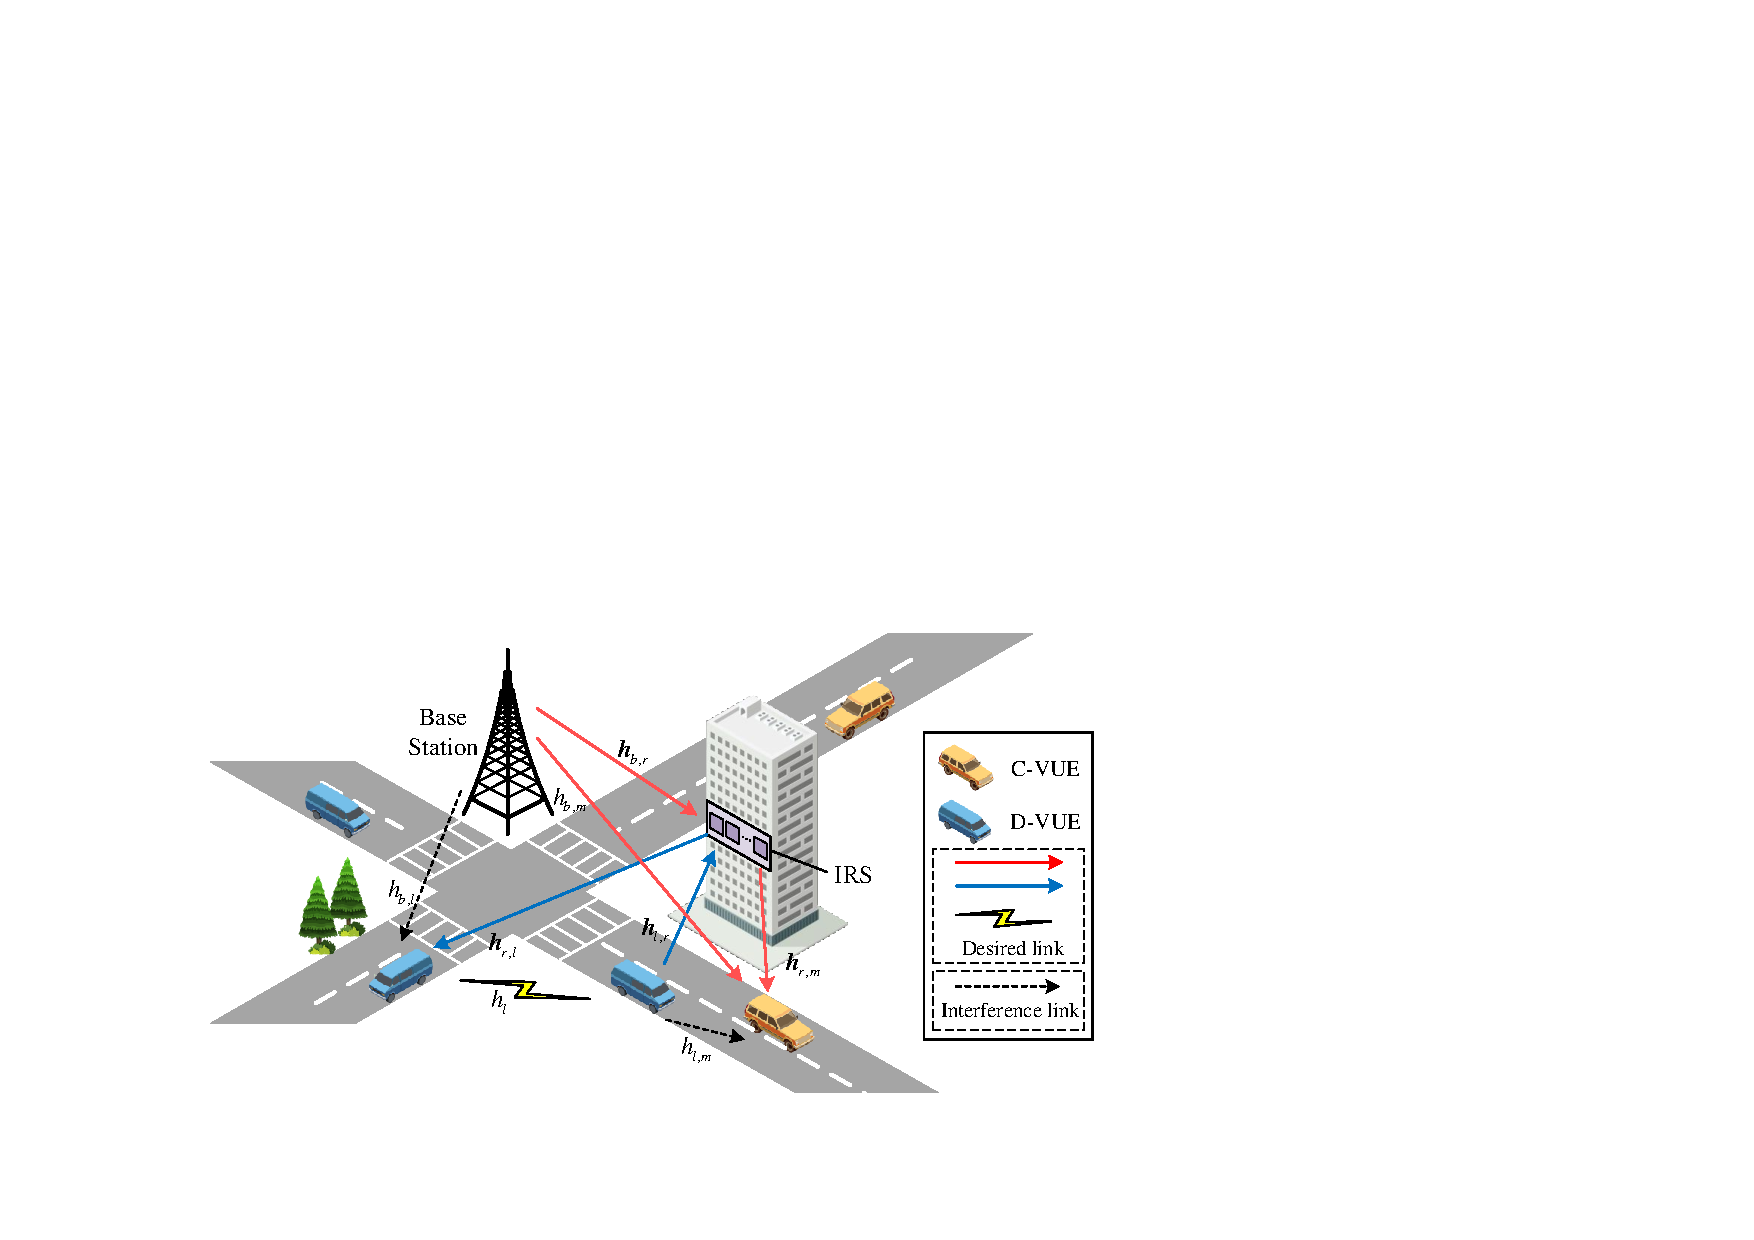
\includegraphics[width=1.0\linewidth]{./plot/Fig1.png}% 1\linewidth
	\caption{RIS-aided Milimeter Wave UAV Communications.}  %\label{fig}
\end{figure}
\subsection{System Model}
In this letter, we consider an RIS-aided milimeter wave UAV secure transmission system where a RIS is exploited to assist the secure downlinks from the UAV to $K$ single-antenna legitimate users in the presence of $P$ single-antenna eavesdroppers. Specifically, the UAV is equipped with an A-element uniform linear array (ULA), and the RIS is a uniform planar array (UPA) with $M=m^2$ passive reflecting elements ($m$ should be an integer). The set of the legitimate users and the eavesdroppers are denoted by ${\cal K}{\rm =}\{ 1,2,...,K \}$,${\cal P}{\rm =}\{1,2,...,P \}$, respectively. As shown in Fig.1, all entities are placed in the three dimensional (3D) Cartesian coordinate system. Let ${\bf{w}}_{k}{\rm{ = }}[x_k,y_k,0]^T,\forall k{\rm \in}{\cal K}$ and ${\bf{w}}_{p}{\rm{ = }}[x_p,y_p,0]^T,\forall p{\rm \in}{\cal P}$ denote the legitimate users' and the eavesdroppers' coordinates, respectively. The RIS is fixed at ${\bf{w}}_{R}{\rm{ = }}[x_R,y_R,z_R]^T$. In addition, assume that the UAV flies at a fixed altitude in a finite time span which is divided into $N$ time slots, i.e., $T{\rm{ = }}N\delta_t$, where $\delta_t$ is the time slot. Then the coordinate of the UAV at the $n$-th time slot is denoted by ${\bf{q}}[n]{\rm{ = }}[x[n],y[n],H_{U}]^T, n \in {\cal N}{\rm{ = }}\{ 1,2,...,N \}$, subject to the following mobility constraints:

\begin{subequations}\label{mobility-1}
	\begin{gather}
  \|\bm{q}[n+1]-\bm{q}[n] \|^2 \leq D^2 , n=1, \ldots, N-1,\\
  \left\lvert x[n] \right\rvert ,\left\lvert y[n] \right\rvert  \leq B , n=1, \ldots, N-1,\\
  \bm{q}[0] \equiv [0,0,H_{U}] , n=1, \ldots, N-1.
	\end{gather}
\end{subequations}

Let ${\bm{h}}_{U,k}\rm{\in} \mathbb{C}^{\emph{A}\times 1},$ $\bm{h}_{U,p} \rm{\in} \mathbb{C}^{\emph{A}\times 1},$ $ \bm{h}_{R,k} \rm{\in} \mathbb{C}^{\emph{M}\times 1},$ $\bm{h}_{R,p} \rm{\in} \mathbb{C}^{\emph{M}\times 1},$ 
$\bm{H}_{UR} \rm{\in} \mathbb{C}^{\emph{M}\times \emph{A}}$ be the channel gains of the UAV to $k$-th user, UAV to $p$-th eavesdropper, RIS to $k$-th user, RIS to $p$-th eavesdropper, UAV to RIS links, respectively. All the channels are modeled as milimeter wave channels~\cite{mmwave-1}\cite{mmwave-2} as 
\begin{subequations}\label{channel-1}
	\begin{align}
  &{\bm{h}}_{U,i}=\sqrt{\frac{1}{L_{UK}}} \sum_{l = 1}^{L_{UK}} g^{u}_{i,l}{\mathbf{a }}_{L}  \left(\theta_{i,l}^{AoD}\right),\forall i \in {\cal K}\cup {\cal P},\\
  &{\bm{h}}_{R,i}=\sqrt{\frac{1}{L_{RK}}} \sum_{l = 1}^{L_{RK}} g^{r}_{i,l}{\mathbf{a }}_{P}  \left(\theta_{i,l}^{AoD}, \phi_{i,l}^{AoD}\right),\forall i \in {\cal K}\cup {\cal P},\\
  &{\bm{h}}_{UR}=\sqrt{\frac{1}{L_{RK}}} \sum_{l = 1}^{L_{RK}} g^{ur}_{l}{\mathbf{a }}_{P}  \left(\theta_{l}^{AoA},\phi_{l}^{AoA}\right){\mathbf{a }}_{L}  \left(\theta_{l}^{AoD}\right)^H .
  \end{align}
\end{subequations}
\noindent In~(\ref{channel-1}), the large-scale fading coefficients defined by  $g \in \{g^u_{i,l},g^{r}_{i,l},g^{ur}_{l}\}$ follow a complex Gaussian distribution as ${\cal CN}(0, 10^{\frac{PL}{10}})$, where $\text{PL(dB)} {\rm =  -C_0-10 \alpha log_{10}(D)-PL_s}$, $C_0{\rm =}61\ \text{dB}$ is the path loss at a reference distance of one meter, $\text{D}\ \text{(meters)}$ is the link distance, $\alpha$ denotes the path-loss exponent, and $\text{PL}_s {\rm \sim} {\cal CN}(0, \sigma_s^2)$ is the shadow fading component. The steering vector of the ULA is denoted by $\mathbf{a}_{L}(\theta)=\left[1, e^{j \frac{2 \pi}{\lambda c} d \sin (\theta)}, \ldots, e^{j \frac{2 \pi}{\lambda c} d(N-1) \sin (\theta)}\right]^{\mathrm{H}}$~\cite{mmwave-4-UPA-ULA}, where $\theta$ stands for the azimuth angle-of-departure(AoD) $\theta_{i,l}^{AoD}$ and $ \theta_{l}^{AoD}$, $d$ is the antenna inter-spacing, and $\lambda_c$ is the carrier wavelength. The steering vector of the UPA is denoted by $\mathbf{a}_{P}(\theta, \phi)=\left[1, \ldots, e^{j \frac{2 \pi}{\lambda c} d(p \sin (\theta) \sin (\phi)+q \cos (\theta) \sin (\phi))}, \ldots\right]^{\mathrm{H}}$~\cite{mmwave-4-UPA-ULA},where $0\leq {p,q}\leq m-1$, $\theta(\phi)$ is the azimuth(elevation) AoD $\theta_{i,l}^{AoD}$($\phi_{i,l}^{AoD}$) and the angle-of-arrival (AoA) $\theta_{l}^{AoA}(\phi_{l}^{AoA})$.

The cascaded channel from the UAV to the $i$-th user or eavesdropper can be written as $ \bm{H}_{C,i}=\text{diag}(\bm{h}_{R,i}^H)\bm{h}_{UR},\forall i \in {\cal K}\cup {\cal P}$. The passive beamforming matrix of the RIS~\cite{passive-beamforming-1} is defined as ${\bf{\Theta }} = {\rm{diag}}\left( {{\beta _1}{e^{j{\theta _1}}},{\beta _2}{e^{j{\theta _2}}},...,{\beta _M}{e^{j{\theta _M}}}} \right)$, where ${\theta _m} \in \left[ {\left. {0,2\pi } \right)} \right.$ and ${\beta _m} \in \left[ {0,1} \right]$ represent the phase shift and amplitude reflection coefficient of the $m$-th RIS reflection element, respectively. For feasibility, the amplitude reflection coefficient subjects to unit-modulus constraints, i.e., ${\beta _m} {\rm =}1 $. Let $\bm{\Psi}{\rm =}\text{vec}(\bf{\Theta})^T $ denote the vectorized passive beamforming matrix. Then, the received signal at the $i$-th user or eavesdropper from the UAV can be formulated as
\begin{equation}\label{received-1}
  y_i=({\bm{h}}_{U,i}^H+{\bm{\Psi}^{H}\bm{H}}_{C,i}){\bf{G}}{\bm{s}}+ {{n}_{i}},\forall i\in {\cal K}\cup{\cal P},
\end{equation}
\noindent where $ s_k$ with $E[|s_k|^2]=1 $ and $ {\bf{G}} \in \mathbb{C}^{\text{A} \times \text{K}}$ represent the transmitted symbol and the beamforming matrix at the UAV, respectively, and it is assumed that $ n_i \sim {\cal N}(0,\sigma_n),\forall i \in {\cal K}\cup {\cal P}$. Let $\bm{g}_k$ be the $k$-th column of the beamforming matrix $\bf{G}$. Then, the the achievable unsecured rate of the $k$-th user is given by
\begin{equation}\label{unsecure-1}
  \begin{aligned}
  &R_k^u = \\
  &{\rm log}_2\left(1+\frac{|(\bm{h}_{U, k}^{H}+\Psi^{H} \bm{H}_{C, k})\bm{g}_k|^2}{\sum_{k^{'} \in {\cal K}\backslash k}  | {}\bm{h}_{U, k}^{H}+\Psi^{H} \bm{H}_{C, k})\bm{g}_{k^{'}} |^2+n_k^2}\right).
  \end{aligned}
\end{equation}
If the $p$-th eavesdropper aims to eavesdrop the signal of the $k$-th user, its achievable rate can be denoted by 
\begin{equation}\label{eavesdrop-1}
  \begin{aligned}
    &R_{p,k}^e = \\
    &{\rm log}_2\left(1+\frac{|(\bm{h}_{U, p}^{H}+\Psi^{H} \bm{H}_{C, p})\bm{g}_k|^2}{\sum_{k^{'} \in {\cal K}\backslash k}  | {}\bm{h}_{U, p}^{H}+\Psi^{H} \bm{H}_{C, p})\bm{g}_{k^{'}} |^2+n_p^2}\right).
  \end{aligned}
\end{equation}
The achievable individual secrecy rate from the UAV to the $k$-th user~\cite{secure-1} can be expressed by
\begin{equation}\label{secure}
  R_{k}^{\mathrm{sec}}=\left[R_{k}^{\mathrm{u}}-\max _{\forall p} R_{p, k}^{\mathrm{e}}\right]^{+}
\end{equation}
where $[z]^{+}=\max (0, z)$.

\newpage
In the practical system, the perfect CSI is not available at the UAV due to the transmission delay and processing delay, as well as the mobility of the UAV and the users. The CSI may be stale at the time when the UAV transmits the data stream to the RIS and the users, which results in an inevitable performance loss once this outdated CSI is employed for transmission. Thus, the outdated CSI should be explicitly considered in the system design.


%It is worth noting that the outdated CSI will lead to substantial performance loss in practical systems. According to~\cite{CSI-error-1}, the outdated CSI can be expressed as statistical CSI error model. 

Let $T_d$ be the delay between the outdated CSI and the real-time CSI. The relation between the outdated channel vector $\bm{h}(t)$ and the real-time channel vector $\bm{h}(t+T_d)$ can be expressed as~\cite{CSI-error-2}
\begin{equation}\label{CSI-error-1}
  \bm{h}\left(t+T_{\text {d }}\right)=\varrho  \tilde{\bm{h}}(t)+\sqrt{1-\varrho^{2}} \Delta \tilde{\bm{h}},
\end{equation}
where $\Delta \tilde{\bm{h}}$ is the error term that is independent identically distributed (i.i.d) with $\bm{h}\left(t+T_{\text {d }}\right)$ and $\tilde{\bm{h}}(t)$, $\varrho $ is the autocorrelation function of the channel gain $\bm{h}(t)$, given by the zeroth-order Bessel function of the first kind as
%\begin{equation}\label{CSI-autocorrelation}
  $ \varrho=J_{0}\left(2 \pi f_{D} T_{\mathrm{d}}\right) $,
%\end{equation}
where $f_D$ is the Doppler spread which is expressed as $f_{D}=v f_{c} / c$, where $v$, $f_c$, $c$ represent the velocity of the transceivers, the carrier frequency and the speed of light, respectively. 

Note that due to the stochastic nature of the error $\Delta \tilde{\bm{h}}$, the error model in (\ref{CSI-error-1}) belongs to statistical error model in essence \cite{CSI-error-1,CSI-error-2}. The autocorrelation function $ \varrho $ bridges the real-time $ \bm{h}\left(t+T_{\text {d }}\right) $ with the estimated $\tilde{\bm{h}}(t)$ that is easily outdated. The actual CSI $ \bm{h} \triangleq \{ \bm{h}_{\mathrm{U}, i},\bm{h}_{\mathrm{R}, i},\bm{h}_{\mathrm{UR}}, \forall i \in \mathcal{K} \cup \mathcal{P}\} $ can be expressed as the form in (\ref{CSI-error-1}). Furthermore, the system can only access to the estimated CSI $ {\tilde{\bm{h}}} \triangleq \{ \tilde{\bm{h}}_{\mathrm{U}, i},\tilde{\bm{h}}_{\mathrm{R}, i},\tilde{\bm{h}}_{\mathrm{UR}}, \forall i \in \mathcal{K} \cup \mathcal{P} \} $\footnote{We assume that the CSI can be obtained by adopting the channel estimation method in the RIS aided system, such as \cite{bibid}.  } that are outdated, and the actual CSI $ \bm{h} $ given by (\ref{CSI-error-1}) is employed to calculate achievable secrecy rate in (\ref{label})-(\ref{label}).


%Then, the actual channel coefficients can be rewritten as 
%\begin{equation}\label{CSI-rewritten}
%  \begin{aligned}
%      \bm{h}_{\mathrm{U}, i} &=\rho\tilde{\bm{h}}_{\mathrm{U}, i}+\Delta \bm{h}_{\mathrm{U}, i}, \forall k \in \mathcal{K}\cup \mathcal{P} ,\\
%      \bm{h}_{\mathrm{R}, i} &=\rho\tilde{\bm{h}}_{\mathrm{R}, i}+\Delta \bm{h}_{\mathrm{R}, i}, \forall k \in \mathcal{K}\cup \mathcal{P} ,\\
%      \bm{h}_{\mathrm{UR}} &=\rho\tilde{\bm{h}}_{\mathrm{UR}}+\Delta \bm{h}_{\mathrm{UR}}.
%  \end{aligned}
%\end{equation}

%Note that the system only has access to the estimated CSI $\tilde{\bm{h}}\in\{ \tilde{\bm{h}}_{\mathrm{U}, i},\tilde{\bm{h}}_{\mathrm{R}, i},\tilde{\bm{h}}_{\mathrm{UR}} \}$, which are outdated, to generate active and passive beamforming and UAV trajectory. And the actual CSI ${\bm{h}}\in\{ {\bm{h}}_{\mathrm{U}, i},{\bm{h}}_{\mathrm{R}, i},{\bm{h}}_{\mathrm{UR}} \}$ is employed to calculate achievable secrecy rate of each user which has been expressed in~(\ref{unsecure-1}),~(\ref{eavesdrop-1}),~(\ref{secure}).
\begin{figure}[t]
	%	Requires \usepackage{graphicx}
	\centering
	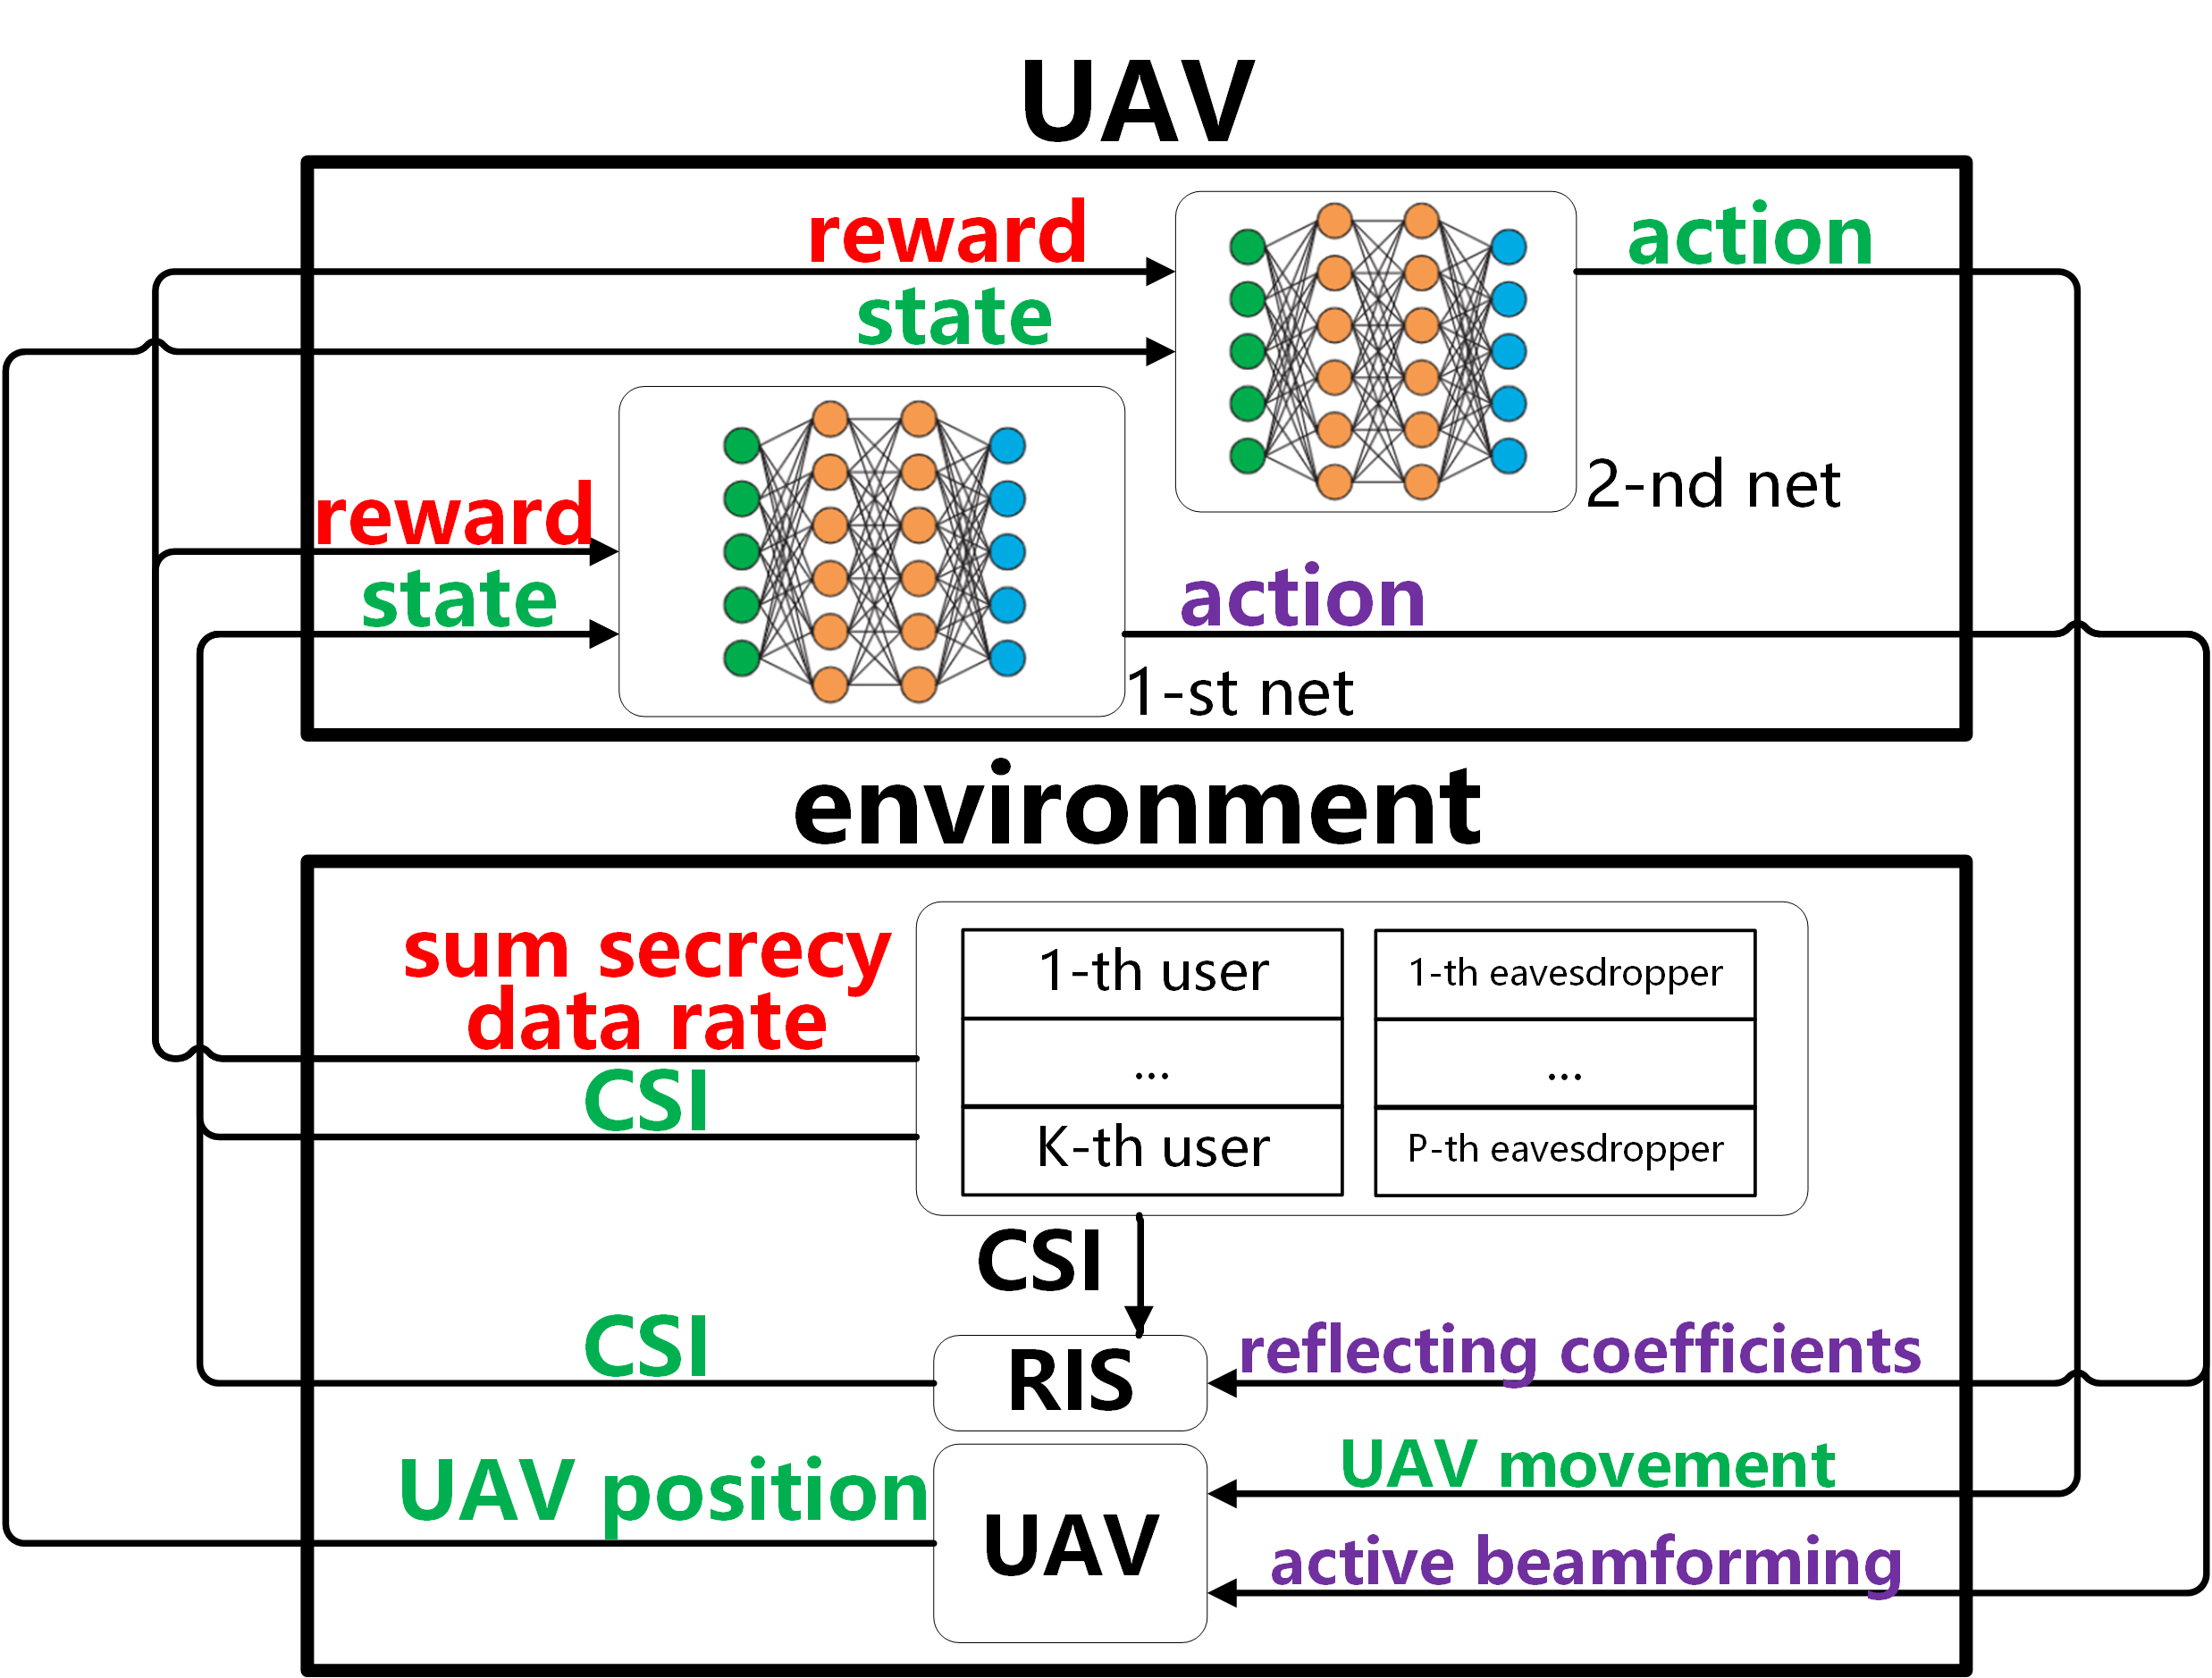
\includegraphics[width=1.0\linewidth]{./plot/construction/construction.png}% 1\linewidth
	\caption{structure of proposed twin-DDPG framwork.}  \label{structure}
\end{figure}
\subsection{Problem Formulation}

In this letter, we aim to maximize the sum secrecy rate $\sum_{k=1}^{K}  R_{k}^{\mathrm{sec}} $ by jointly optimizing the UAV's trajectory $\bf{Q} \triangleq\{\bm{q}[n], n \in \mathcal{N}\}$ and the active (passive) beamforming matrix $\bf{G}$($\bf{\Theta}$). The optimization problem is formulated as 
\begin{subequations}\label{formulation}
  \begin{align}
    &\mathop {\max }\limits_{{\bf{Q}},{\bf{G}},{\bf{\Theta }}} \quad\sum\limits_{k \in {\cal K}} {{R_k^{\mathrm{sec}}}}\\
    s.t.\qquad &(\ref{mobility-1}),\\
    &\operatorname{Pr}\left\{{R_k^{\mathrm{sec}}} \geq R_{k}^{\mathrm{sec,th}}\right\} \geq 1-\rho_{k}, \forall k \in \mathcal{K},\\
    &\operatorname{Tr}\left(\bf{G} \bf{G}^{H}\right) \leq P_{\max },\\
    &{\theta _m} \in \left[ {\left. {0,2\pi } \right)} \right. , \forall m \in {\cal M},
  \end{align}
\end{subequations}
where the rate outage constraint in~(\ref{formulation}\rm{c}) guarantees that the probability that each legitimate user can successfully decode its message at a data rate of $ R_{k}^{\mathrm{sec,th}}$ is no less than $1-\rho_k$. ~(\ref{formulation}\rm{b}) models the UAV mobility constraint. ~(\ref{formulation}\rm{d}) restricts the transmission power at UAV side does not exceed the maximum value. ~(\ref{formulation}\rm{e}) constrains the reflection coefficients of  the RIS reflecting elements. Obviously, problem~(\ref{formulation}), due to the non-convex objective function and constraints, is a non-convex problem that is rather challenging to solve. To tackle this challenging problem, the sum rate optimization problem is formulated in the context of DRL based method to obtain the feasible $\bf{G} $, $\bf{\Theta} $ and $\bf{Q}$.
\section{DRL-based Solution}
To solve the non-convex problem in~(\ref{formulation}), we propose a twin-DDPG deep reinforcement learning framwork, instead of using single agent to find the optimal $\bf{G} $, $\bf{\Theta} $ and $\bf{Q}$, since $\bf{Q}$ would be highly coupled with large scale CSI using single agent which is actually irrelevant. As shown in Fig.2, the first network takes CSI as state to obtain the optimal $\bf{G} $ and $\bf{\Theta} $, while the second network takes UAV position as state to obtain the movement $\bf{q}[n+1]-\bf{q}[n]$ of UAV at $n$-th time slot. Both network take the sum secrecy data rate as reward. The overall algorithm for solving problem~(\ref{formulation}) is summarized in Algorithm 1.
\begin{algorithm}[t]
	\caption{Twin-DDPG Deep Reinforcement Learning Algorithm}
	\begin{algorithmic}[1]
    \STATE {Initialize the 1-st network with initial Q-function $Q_1(s,a;\bm{\theta}_1)$;}
    \STATE {Initialize the 2-nd network with initial Q-function $Q_2(s,a;\bm{\theta}_2)$;}
    \FOR {Episode $n_{ep} = 1,2,...,N_{ep}$}
      \STATE {Reset the positions of the UAV and users;}
      \STATE{Reset the active and passive beamforming matrix $\bf{G}$, $\bf{\Theta}$; }
      \FOR {Step $n = 1,2,...,N_{step}$}
        \STATE{Observe all CSI as $s_{n,1}$;}
        \STATE{Observe the UAV position as $s_{n,2}$;}
        \STATE{Select actions $a_{n,1},a_{n,2}$ with a gaussian action noise $n_{a}$ with variance $\sigma_a$ :}
        \begin{equation}
          \begin{aligned}
            a_{n,1}=\arg \max _{a_{n,1} \in \mathcal{A}} Q_1\left(s_{n,1}, a_{n,1} ; \theta_{n,1}\right)+n_{a}\\
            a_{n,2}=\arg \max _{a_{n,2} \in \mathcal{A}} Q_2\left(s_{n,2}, a_{n,2} ; \theta_{n,2}\right)+n_{a}
          \end{aligned}            
        \end{equation}
        \STATE{Execute action $a_{n,1},a_{n,2}$, receive an immediate reward $r_{n,1}$ using Eq.~(\ref{reward}) and new states $s_{n+1,1},s_{n+1,2}$. Note that $r_{n,1}=r_{n,2}$;}
        \STATE{Store the transitions $[s_{n,1},a_{n,1},r_{n,1},s_{n+1,1}]$ and $[s_{n,2},a_{n,2},r_{n,2},s_{n+1,2}]$ in the two networks' memory queues, respectively;}
        \STATE{Sample a mini-batch of transitions in memory queue randomly to update both networks using proper loss function and policy gradient function~\cite{RL-4};}
      \ENDFOR
    \ENDFOR
	\end{algorithmic}
\end{algorithm}

\subsection{Active and Passive Beamforming}
Inspired by the work of~\cite{secure-1}, a DDPG-based network is employed to learn the optimal policy in terms of the UAV's beamforming matrix $\bf{G}$ and the RIS's reflecting beamforming matrix $\bf{\Theta}$ by interacting with the whole system. Each episode is defined as a time span $T$, where each step is defined as a time slot $\delta_n$. In order to maximize the sum secrecy rate, the state $s_{n,1}$, the action $a_{n,1}$, the reward $r_{n,1}$ in $n$-th time slot of the first agent is defined as follows:
\begin{itemize}
  \item [1)] 
  State $s_{n,1}$: the state of the first agent in $n$-th time slot contains the estimated comprehensive CSI from the UAV to all legitimate users and eavesdroppers, i.e., $\{ \bf{h}_{U,i}^{H}+\bm{\Psi}^{H}\bf{H}_{C,i} \},\forall i \in {\cal K}\cup {\cal P} $ .
  \item [2)]
  Action $a_{n,1}$: we define the phase shift of all RIS reflecting elements $\theta_n, \forall n \in {\cal N}$ and the transmit beamforming matrix $G $ as action. It is worth noting that $\bf{G} = Re\{ \bf{G} \} + Im\{ \bf{G} \}$ are separated as real part and imaginary part to tackle with the real input problem.
  \item [3)]
  Reward $r_{n,1}$: the reward function is defined as:
  \begin{equation}\label{reward}
    r_{n,1}=tanh(\sum_{k=1}^{K}  R_{k}^{\mathrm{sec}}-p_{r}-p_{m}),
  \end{equation}
  where $p_{r}$ is the penalty if the outage constraint~(\ref{formulation}\rm{c}) is not satisfied, and $p_{m}$ is the the penalty when the UAV flies out of the target area. The hyperbolic tangent function $tanh(\cdot )$ is exploited to limite reward in range of $(-1,1)$ for better convergence.
\end{itemize}
\subsection{UAV Trajectory}
The second DDPG is exploited to simultaneously obtain the optimal movement $\bf{q}[n+1]-\bf{q}[n]$ with $\bf{G}$ and $\bf{\Theta}$. It is feasible to utilize a single DDPG network to tune all parameters $\bf{G}, \bf{\Theta}, \bf{Q}$, which have been done by most works. But in this letter, UAV's trajectory is rarely relevant to the large amount of CSI, leading to instability and divergence by connecting irrelevant actions and feedbacks using a single network. The state $s_{n,2}$, the action $a_{n,2}$, the reward $r_{n,2}$ in $n$-th time slot of the second agent is defined as follows:
\begin{itemize}
  \item [1)] 
  State $s_{n,2}$: as mentioned before, UAV's trajectory is rarely relevant to the large amount of CSI. So the second network only takes the UAV's position $\bf{q}[n]$ as state.
  \item [2)]
  Action $a_{n,2}$: the action contains the UAV's flying distance $\mu[n] $ and the direction $\psi[n] $. Then, the movement of UAV can be expressed as:
  \begin{equation}
    \bf{q}[n+1]-\bf{q}[n]=\mu[n](cos\psi[n] \bf{e}_x+ sin\psi[n] \bf{e}_y)
  \end{equation}
  \item [3)]
  Reward $r_{n,2}$: the same reward function in~(\ref{reward}) is employed, since both network have the same objective to maximize the sum secrecy rate.
\end{itemize}

\subsection{omputational Complexity Analysis}

\section{Simulation Results}
In this section, numerical results are presented to characterize the performance of our proposed solution. For the first DDPG-based network, we deploy four fully-connected hidden layers with [800,600,512,256] neurons in both actor and critic networks and the AdamOptimizer is used to train the actor network with learning rate 0.0001 and critic network with learning rate 0.001. The second net has the same structure as the first net, but with different number of four layers [400,300,256,128]. The initial coordinates of UAV and RIS are set as [0,25,50], [0,50,12.5]. The eavesdropper is placed at [47,-4,0], while we model two legitimate users' movement as uniform motion in a straight line as shown in Fig.\ref{trajectory}. More parameters are shown in Tabel. \uppercase\expandafter{\romannumeral1}.

\begin{table}
  \centering
  \caption{Main Parameters.}
  \begin{tabular}{cc} 
  \toprule
  Parameter              & Value    \\ 
  \hline
  UAV antennas number    &${\bf{A}}=4$        \\
  eavesdropper number    &${\bf{P}} = 1$        \\
legitimate user number &${\bf{K}} =2$        \\
  step number            & $N_{step}=100$      \\
  episode number         & $N_{ep}=100$      \\
  carrier frequency      &$f_c=28\ \text{GHz}$\\
  max transmission power            &$P_{max }= 30\ \text{dBm}$  \\
  noise power            &$\sigma_n= -114\ \text{dBmW}$  \\
  path loss factor\cite{parameters}       &    $\alpha_{ur}=2.2,\alpha_{u}=3.5,\alpha_{r}=2.8$      \\
  shadow   fading factor &$\sigma_s = 3\ \text{dB} $     \\
  \bottomrule
  \end{tabular}
\end{table}

\begin{figure}
  \centering
	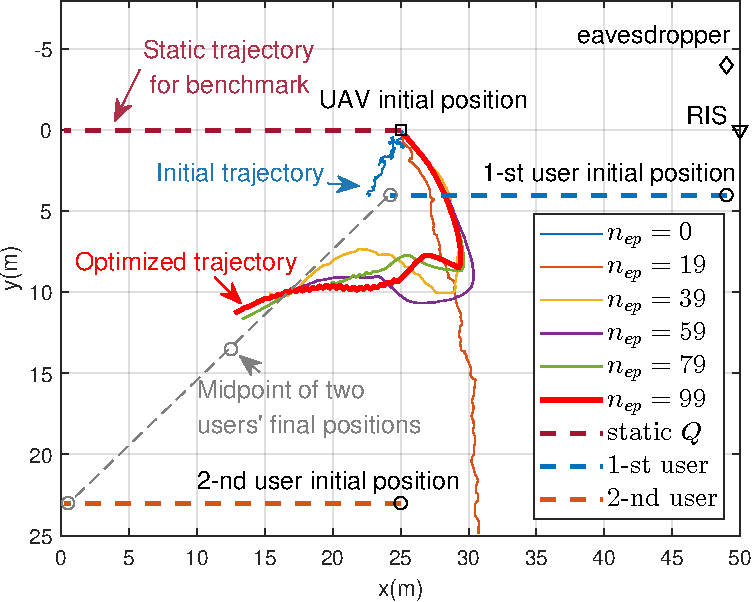
\includegraphics[width=1.0\linewidth]{./plot/trajectory/trajectory.pdf}% 1\linewidth
	\caption{Converged trajectory of the UAV.}  %\label{fig}
  \label{trajectory}
\end{figure}
Fig.\ref{trajectory} illustrates the optimized trajectory, which eventually converges as the learning procedure is over. It can be observed that the UAV tends to move away from the eavesdropper. Moreover, the UAV is inclined to chase and follow the midpoint of two users position, while keeping relatively close distance to the RIS. This implies the UAV trajectory is jointly optimized with the active and passive beamforming, and the proposed algorithm can adapt to dynamic conditions brought by the users' mobility.

\begin{figure}
  \centering
	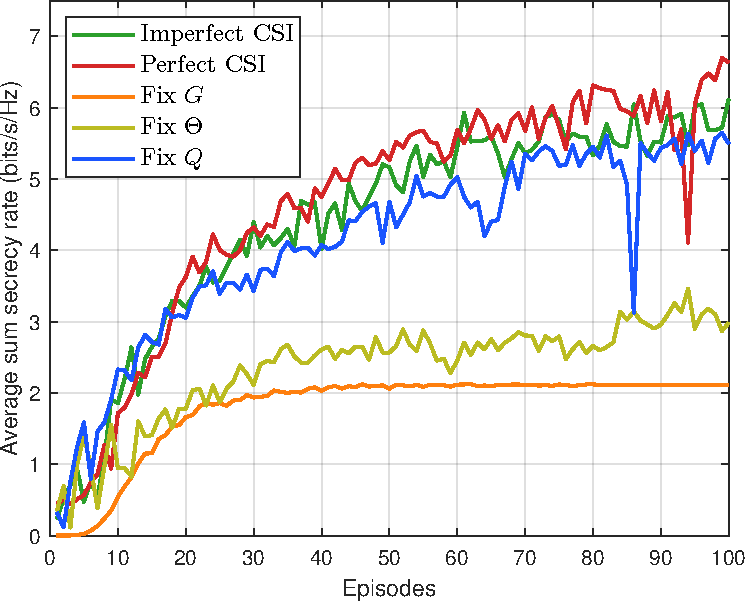
\includegraphics[width=1.0\linewidth]{./plot/compare/compare.pdf}% 1\linewidth
	\caption{Accumulated reward performance versus episodes under different RIS elements number.}  %\label{fig}
  \label{compare}
\end{figure}
Fig.\ref{compare} plots the average sum secrecy rate by different benchmarks which all increase with traning episode $n_{ep}$. It is found that the proposed solution which jointly optimizes UAV trajectory and active (passice) beamforming achieves the best performance under imperfect CSI, compared with other benchmarks which fix UAV trajectory, active beamforming and passive beamforming, respectively. However, the proposed solution performs slightly better under the perfect CSI, which implies the proposed solution has good robustness. Thus, the secrecy rates of legitimate users in our proposed system under imperfect CSI can be maximized leveraging RIS and UAV by proposed DDPG-based algorithm.

\section{Conclusion}
In this letter, we investigated robust and secure transmission for RIS-aided mmWave UAV communications. To maximize the secrecy rates of legitimate users, we proposed a DDPG-baesd optimization algorithm. The simulation results validated that by jointly optimizing UAV trajectory and active (passice) beamforming, the best performance can be achieved under imperfect CSI compared with other benchmarks.





% if have a single appendix:
%\appendix[Proof of the Zonklar Equations]
% or
%\appendix  % for no appendix heading
% do not use \section anymore after \appendix, only \section*
% is possibly needed

% use appendices with more than one appendix
% then use \section to start each appendix
% you must declare a \section before using any
% \subsection or using \label (\appendices by itself
% starts a section numbered zero.)
%


%\appendices
%\section{Proof of the First Zonklar Equation}
%Appendix one text goes here.

% you can choose not to have a title for an appendix
% if you want by leaving the argument blank
%\section{}
%Appendix two text goes here.


% use section* for acknowledgment
%\section*{Acknowledgment}


%The authors would like to thank...


% Can use something like this to put references on a page
% by themselves when using endfloat and the captionsoff option.
%\ifCLASSOPTIONcaptionsoff
%  \newpage
%\fi



% trigger a \newpage just before the given reference
% number - used to balance the columns on the last page
% adjust value as needed - may need to be readjusted if
% the document is modified later
%\IEEEtriggeratref{8}
% The "triggered" command can be changed if desired:
%\IEEEtriggercmd{\enlargethispage{-5in}}

% references section

% can use a bibliography generated by BibTeX as a .bbl file
% BibTeX documentation can be easily obtained at:
% http://mirror.ctan.org/biblio/bibtex/contrib/doc/
% The IEEEtran BibTeX style support page is at:
% http://www.michaelshell.org/tex/ieeetran/bibtex/
%\bibliographystyle{IEEEtran}
% argument is your BibTeX string definitions and bibliography database(s)
%\bibliography{IEEEabrv,../bib/paper}
%
% <OR> manually copy in the resultant .bbl file
% set second argument of \begin to the number of references
% (used to reserve space for the reference number labels box)

\bibliographystyle{IEEEtran}
\bibliography{WCL_v1_ref}                        %ref为.bib文件名
% biography section
% 
% If you have an EPS/PDF photo (graphicx package needed) extra braces are
% needed around the contents of the optional argument to biography to prevent
% the LaTeX parser from getting confused when it sees the complicated
% \includegraphics command within an optional argument. (You could create
% your own custom macro containing the \includegraphics command to make things
% simpler here.)
%\begin{IEEEbiography}[{\includegraphics[width=1in,height=1.25in,clip,keepaspectratio]{mshell}}]{Michael Shell}
% or if you just want to reserve a space for a photo:

%\begin{IEEEbiography}{Michael Shell}
%Biography text here.
%\end{IEEEbiography}

% if you will not have a photo at all:
%\begin{IEEEbiographynophoto}{John Doe}
%Biography text here.
%\end{IEEEbiographynophoto}

% insert where needed to balance the two columns on the last page with
% biographies
%\newpage

%\begin{IEEEbiographynophoto}{Jane Doe}
%Biography text here.
%\end{IEEEbiographynophoto}

% You can push biographies down or up by placing
% a \vfill before or after them. The appropriate
% use of \vfill depends on what kind of text is
% on the last page and whether or not the columns
% are being equalized.

%\vfill

% Can be used to pull up biographies so that the bottom of the last one
% is flush with the other column.
%\enlargethispage{-5in}



% that's all folks
\end{document}


